\documentclass[journal,12pt,twocolumn]{IEEEtran}

\usepackage{setspace}
\usepackage{gensymb}
\singlespacing
\usepackage[cmex10]{amsmath}

\usepackage{amsthm}
\usepackage{lipsum,adjustbox}
\usepackage{mathrsfs}
\usepackage{txfonts}
\usepackage{stfloats}
\usepackage{bm}
\usepackage{cite}
\usepackage{cases}
\usepackage{subfig}

\usepackage{longtable}
\usepackage{multirow}
\usepackage{adjustbox}
\usepackage{enumitem}
\usepackage{mathtools}
\usepackage{steinmetz}
\usepackage{tikz}
\usepackage{circuitikz}
\usepackage{verbatim}
\usepackage{tfrupee}
\usepackage[breaklinks=true]{hyperref}
\usepackage{graphicx}
\usepackage{tkz-euclide}
\usepackage{tikz}
\usetikzlibrary{shapes.multipart}

\usetikzlibrary{calc,math}
\usepackage{listings}
    \usepackage{color}                                            %%
    \usepackage{array}                                            %%
    \usepackage{longtable}                                        %%
    \usepackage{calc}                                             %%
    \usepackage{multirow}                                         %%
    \usepackage{hhline}                                           %%
    \usepackage{ifthen}                                           %%
    \usepackage{lscape}     
\usepackage{multicol}
\usepackage{chngcntr}

\DeclareMathOperator*{\Res}{Res}

\renewcommand\thesection{\arabic{section}}
\renewcommand\thesubsection{\thesection.\arabic{subsection}}
\renewcommand\thesubsubsection{\thesubsection.\arabic{subsubsection}}
% \renewcommand{\thefigure}{\theenumi}
\renewcommand\thesectiondis{\arabic{section}}
\renewcommand\thesubsectiondis{\thesectiondis.\arabic{subsection}}
\renewcommand\thesubsubsectiondis{\thesubsectiondis.\arabic{subsubsection}}
\usepackage{tikz}
\usetikzlibrary{shapes,arrows}

\hyphenation{op-tical net-works semi-conduc-tor}
\def\inputGnumericTable{}                                 %%

\lstset{
%language=C,
frame=single, 
breaklines=true,
columns=fullflexible
}
\begin{document}


\newtheorem{theorem}{Theorem}[section]
\newtheorem{problem}{Problem}
\newtheorem{proposition}{Proposition}[section]
\newtheorem{lemma}{Lemma}[section]
\newtheorem{corollary}[theorem]{Corollary}
\newtheorem{example}{Example}[section]
\newtheorem{definition}[problem]{Definition}

\newcommand{\BEQA}{\begin{eqnarray}}
\newcommand{\EEQA}{\end{eqnarray}}
\newcommand{\define}{\stackrel{\triangle}{=}}
\bibliographystyle{IEEEtran}
\raggedbottom
\setlength{\parindent}{0pt}
\providecommand{\mbf}{\mathbf}
\providecommand{\pr}[1]{\ensuremath{\Pr\left(#1\right)}}
\providecommand{\qfunc}[1]{\ensuremath{Q\left(#1\right)}}
\providecommand{\sbrak}[1]{\ensuremath{{}\left[#1\right]}}
\providecommand{\lsbrak}[1]{\ensuremath{{}\left[#1\right.}}
\providecommand{\rsbrak}[1]{\ensuremath{{}\left.#1\right]}}
\providecommand{\brak}[1]{\ensuremath{\left(#1\right)}}
\providecommand{\lbrak}[1]{\ensuremath{\left(#1\right.}}
\providecommand{\rbrak}[1]{\ensuremath{\left.#1\right)}}
\providecommand{\cbrak}[1]{\ensuremath{\left\{#1\right\}}}
\providecommand{\lcbrak}[1]{\ensuremath{\left\{#1\right.}}
\providecommand{\rcbrak}[1]{\ensuremath{\left.#1\right\}}}
\theoremstyle{remark}
\newtheorem{rem}{Remark}
\newcommand{\sgn}{\mathop{\mathrm{sgn}}}
% \providecommand{\abs}[1]{\left\vert#1\right\vert}
% \providecommand{\res}[1]{\Res\displaylimits_{#1}} 
% \providecommand{\norm}[1]{\left\lVert#1\right\rVert}
% %\providecommand{\norm}[1]{\lVert#1\rVert}
% \providecommand{\mtx}[1]{\mathbf{#1}}
% \providecommand{\mean}[1]{E\left[ #1 \right]}
\providecommand{\fourier}{\overset{\mathcal{F}}{ \rightleftharpoons}}
%\providecommand{\hilbert}{\overset{\mathcal{H}}{ \rightleftharpoons}}
\providecommand{\system}{\overset{\mathcal{H}}{ \longleftrightarrow}}
	%\newcommand{\solution}[2]{\textbf{Solution:}{#1}}
\newcommand{\solution}{\noindent \textbf{Solution: }}
\newcommand{\cosec}{\,\text{cosec}\,}
\providecommand{\dec}[2]{\ensuremath{\overset{#1}{\underset{#2}{\gtrless}}}}
\newcommand{\myvec}[1]{\ensuremath{\begin{pmatrix}#1\end{pmatrix}}}
\newcommand{\mydet}[1]{\ensuremath{\begin{vmatrix}#1\end{vmatrix}}}
\numberwithin{equation}{subsection}

\makeatletter
\@addtoreset{figure}{problem}
\makeatother
\let\StandardTheFigure\thefigure
\let\vec\mathbf
\renewcommand{\thefigure}{\theproblem}
\def\putbox#1#2#3{\makebox[0in][l]{\makebox[#1][l]{}\raisebox{\baselineskip}[0in][0in]{\raisebox{#2}[0in][0in]{#3}}}}
     \def\rightbox#1{\makebox[0in][r]{#1}}
     \def\centbox#1{\makebox[0in]{#1}}
     \def\topbox#1{\raisebox{-\baselineskip}[0in][0in]{#1}}
     \def\midbox#1{\raisebox{-0.5\baselineskip}[0in][0in]{#1}}
\vspace{3cm}
\title{Assignment 1}
\author{Piyush Kumar Uttam - EE18BTECH11036}
\maketitle
\newpage
\bigskip
\renewcommand{\thefigure}{\theenumi}
\renewcommand{\thetable}{\theenumi}
Download all latex-tikz codes from 
%
\begin{lstlisting}
https://github.com/piyushSTK/C-DS/blob/main/Assignment1/assignment1.tex
\end{lstlisting}
\setcounter{figure}{0}
\section{Problem}
(Q 26) Consider the following C function.
\begin{lstlisting}
void convert(int n){
    if(n<0) printf("%d", n);
    else{
        convert(n/2);
        printf("%d", n%2);
    }
}
\end{lstlisting}
\setcounter{figure}{0}
Which of the following will happen when the function \textbf{convert} is called with any positive integer n as argument?
\begin{enumerate}
    \item It will print the binary representation of \textbf{n} and terminate.
    \item It will print the binary representation of \textbf{n} in the reverse order and terminate.
    \item It will print the binary representation of \textbf{n} and will not terminate.
    \item It will not print anything and will not terminate.
\end{enumerate}

\section{Solution}
Answer : D) It will not print anything and will not terminate.
\newline
\textbf{Explanation}
\newline
This is a problem involving recursion, as $n>0$ the portion 

\begin{lstlisting}
    else{
        convert(n/2);
        printf("%d", n%2);
    }
\end{lstlisting}
\setcounter{figure}{0}
will be evaluated. In this portion, convert is called again with value of \textbf{n/2} and subsequently \textbf{n} goes from $n -> 0$.
\newline
\newline
\newline
\newline
However as \textbf{n} = 0; the condition 
\newline
\begin{lstlisting}
    if(n<0) printf("%d", n);
\end{lstlisting}
\setcounter{figure}{0}
is still not satisfied and $0/2 = 0$. Hence it will not terminate and will not print anything as print statement is after \textbf{convert(n/2)} call.




\section{Problem}
Obtain a new code to get option 1.
\newline
\textbf{Solution}
\newline
The first option can be found using the following piece of code.

\begin{lstlisting}
void convert(int n){
    if(n<=0) return;
    else{
        convert(n/2);
        printf("%d", n%2);
    }
}

\end{lstlisting}
\setcounter{figure}{0}

The flowchart for the given problem is given in the \nameref{Figures} section.
\tikzstyle{decision} = [diamond, draw, fill=white!20, 
    text width=4.5em, text badly centered, node distance=3cm, inner sep=0pt]
\tikzstyle{block} = [rectangle, draw, fill=white!20, 
    text width=7em, text centered, rounded corners, minimum height=1em]
\tikzstyle{line} = [draw, -latex']
\tikzstyle{cloud} = [draw, ellipse,fill=red!20, node distance=3cm,
    minimum height=2em]
\tikzstyle{smblock} = [rectangle, draw, fill=white!20, 
    text width=4em, text centered, rounded corners, minimum height=1em]






\section{Problem}
Obtain a new code using only for loops.
\newline
\textbf{Solution}
\newline
Getting binary representation using only for loop can be found in following piece of code.
The given code uses only 2 int variables to remove the need for additional stack memory.
\newpage
\begin{lstlisting}
void convert(int n){
    if(n == 0){
        printf("%d", 0);
    }
    int p = floor(log2(n));
    int div = pow(2,p);
    for(int i = p; i>=0; i--){
        if(n - div>=0){
            printf("%d", 1);
            n = n-div;
            div = div/2;
        }
        else{
            printf("%d", 0);
            div = div/2;
        }
    }
    return;
}
\end{lstlisting}
\setcounter{figure}{0}

\section{Problem}
Explain which method is better out of recursion and iteration.
\newline
\textbf{Solution}
\newline
Using iterative method is better than using recursion for the following reasons:
\begin{enumerate}
  \item Recursion utilizes call stack where all the local variables and return addresses are stored in a stack frame above the previous recursive call's stack frame.
  \item It generally uses more memory than optimised iterative program.
  \item Stack overflow is a common error which recursive functions encounter. This happens when the number of recursive calls exceed the allocated stack memory limit.
  \item So since time complexity is same for both solutions, hence iterative solution with lesser space usage is better approach.
\end{enumerate}
The visualisation of recursive solution stack memory diagram and iterative solution stack memory diagram is given in the \nameref{Figures}
 section.

\newpage

\section{Problem}
Derive the time complexity of the original solution.
\newline
\textbf{Solution}
\newline
Let's assume the time taken to process the given input N to be $T(n)$ .
\newline
So time taken to process N/2 will be $T(n/2)$
\newline
Lets assume print() function takes some constant C time to process.
\newline Therefore from the program we can see that:
\begin{equation} \label{eq1}
\begin{split}
T\brak{n} = T\brak{n/2} + C\\
\end{split}
\end{equation}
and
\begin{equation} \label{eq2}
\begin{split}
T\brak{n/2} = T\brak{n/4} + C\\
\end{split}
\end{equation}
Substituting equation \eqref{eq2} in \eqref{eq1} we get

\begin{equation} \label{eq3}
\begin{split}
T\brak{n} = T\brak{n/4} + C + C\\
\end{split}
\end{equation}
On repeated substitution till n $->$ 0 we get:

\begin{equation} 
\begin{split}
T\brak{n} = T\brak{0} + C + C + C + C ...... log_{2}(n) times \\
\end{split}
\end{equation}

\begin{flalign}
&\implies T\brak{n} = C*log_{2}(n) + T\brak{0} & \\
&\implies T\brak{n} \leqslant C*log_{2}(n) & \\
&\implies T\brak{n} \in \mathcal{O}\brak{log(n)}&
\end{flalign}

Hence the program has logarithmic time complexity.
\newpage
\setcounter{figure}{0}
\section{Figures}
\label{Figures}




\begin{figure}[!h]
\centering
\begin{adjustbox}{width=\textwidth}
\begin{tikzpicture}[node distance = 2cm, auto]
    % Place nodes
    \node [cloud] (start) {start};
    \node [block, below of=start] (init1) {convert(n)};
    \node [decision, below of=init1] (decision1) { $n<=0$ ? };
    \node [block, below of=decision1, node distance=4cm] (print1) {print(n \% 2)};
    \node [block, below of=print1] (return1) {return};
    \node [smblock, right of=decision1, node distance=3cm] (nextN1) {n = n/2};
    \node [cloud, below of=return1] (end) {end};
    
    \node [block, right of=init1, node distance=6.2cm] (init2) {convert(n)};
    \node [decision, below of=init2] (decision2) { $n<=0$ ? };
    \node [block, below of=decision2, node distance=4cm] (print2) {print(n \% 2)};
    \node [smblock, right of=decision2, node distance=3cm] (nextN2) {n = n/2};
    \node [block, below of=print2] (return2) {return};
    
    \node [block, right of=init2, node distance=6.2cm] (init3) {convert(n)};
    \node [decision, below of=init3] (decision3) { $n<=0$ ? };
    \node [block, below of=decision3, node distance=4cm] (print3) {print(n \% 2)};
    \node [block, right of=decision3, node distance=3.6cm] (nextN3) {next recursion};
    \node [block, below of=print3] (return3) {return};
    \node [block, right of=return3, node distance=3.6cm] (retN3) {next recursion};

    % Draw edges
    \path [line] (start) -- (init1);
    \path [line] (init1) -- (decision1);
    \path [line] (decision1) -- node [near start] {no} (nextN1);

    \path [line] (nextN1) |- (init2);
    \path [line] (init2) -- (decision2);
    \path [line] (decision2) -- node [near start] {no} (nextN2);
    \path [line] (nextN2) |- (init3);
    \path [line] (init3) -- (decision3);
    \path [line] (decision3) -- node [near start] {no} (nextN3);

    \path [line, dashed] (return2) |- ++(-3,-1) |-  (print1);
    \path [line, dashed] (return3) |- ++(-3,-1) |-  (print2);
    \path [line, dashed] (retN3) |-  (print3);
    \path [line] (print1) -- (return1);
    \path [line] (return1) -- (end);
    \path [line] (print2) -- (return2);
    \path [line] (print3) -- (return3);
    \path [line] (decision1)  -- ++(-2,0) |-  node[pos=.25]{yes}  (return1);
    \path [line] (decision2)  -- ++(-2,0) |-  node[pos=.25]{yes}  (return2);
    \path [line] (decision3)  -- ++(-2,0) |-  node[pos=.25]{yes}  (return3);
    % \path [line] (evaluate) -- (decide);
    % \path [line] (decide) -| node [near start] {yes} (update);
    % \path [line] (update) |- (identify);
    % \path [line] (decide) -- node {no}(stop);
    % \path [line,dashed] (expert) -- (init);
    % \path [line,dashed] (system) -- (init);
    % \path [line,dashed] (system) |- (evaluate);
\end{tikzpicture}

\end{adjustbox}
\caption{Flowchart of recursive calls of convert(n)} \label{fig:M1}
\end{figure}

\clearpage


\begin{figure}[!h]
\centering
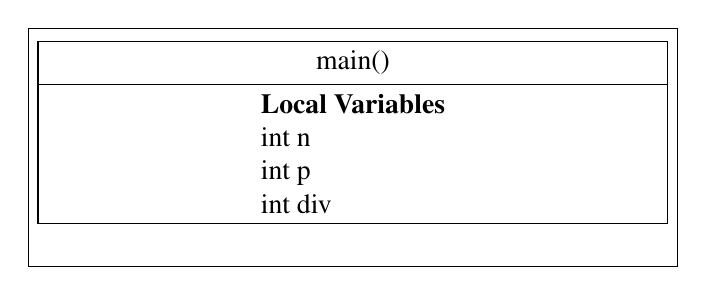
\begin{tikzpicture}[
  double/.style={draw, anchor=text, rectangle split,rectangle split parts=2, minimum height=6cm,minimum width=8cm},
  triple/.style={draw, anchor=text, rectangle split,rectangle split parts=3},
  single/.style={draw, anchor=text, rectangle split,rectangle split parts=1, minimum height=6cm,minimum width=8cm}
  ]
    
  \node[single,align=center] {

        \\
        \tikz{\node[double,align=left] {main()\nodepart{second}  \textbf{Local Variables}\\ int n\\int p\\int div};}\\
  };

\end{tikzpicture}
    \caption{Stack memory diagram for iterative solution}
    \label{fig:iterStack}

\end{figure}
\begin{figure}[!h]
\centering
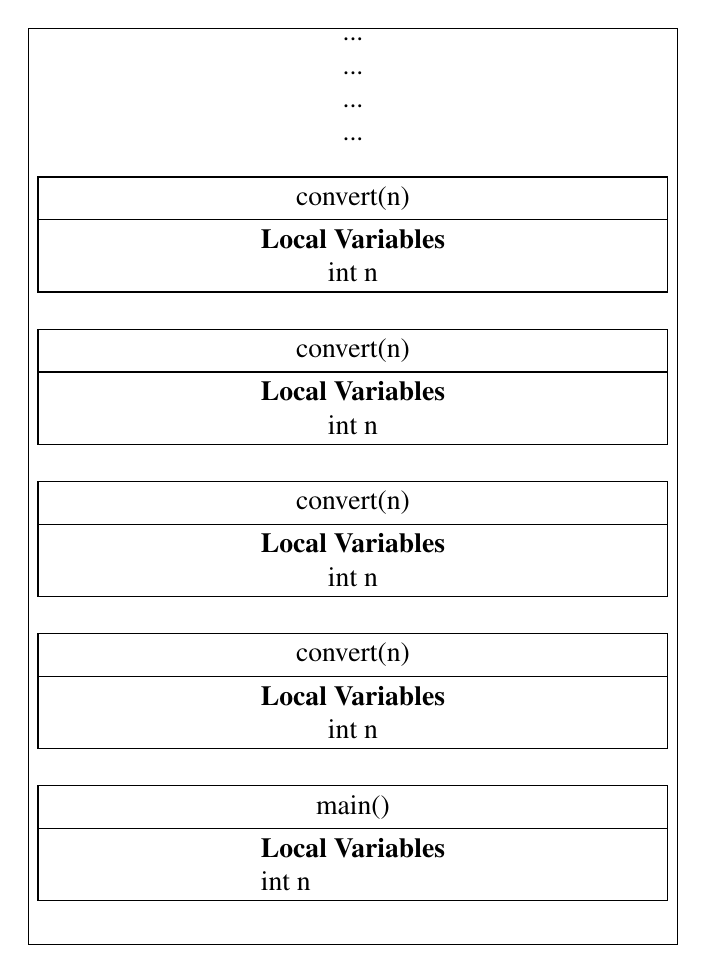
\begin{tikzpicture}[
  double/.style={draw, anchor=text, rectangle split,rectangle split parts=2, minimum height=6cm,minimum width=8cm},
  triple/.style={draw, anchor=text, rectangle split,rectangle split parts=3},
  single/.style={draw, anchor=text, rectangle split,rectangle split parts=1, minimum height=6cm,minimum width=8cm}
  ]
    
  \node[single,align=center] {
        ...\\
        ...\\
        ...\\
        ...\\
        \\
        \tikz{\node[double,align=center] {convert(n)\nodepart{second}\textbf{Local Variables}\\ int n};}\\
        \\
        \tikz{\node[double,align=center] {convert(n)\nodepart{second}\textbf{Local Variables}\\ int n};}\\
        \\        
        \tikz{\node[double,align=center] {convert(n)\nodepart{second}\textbf{Local Variables}\\ int n};}\\
        \\
        \tikz{\node[double,align=center] {convert(n)\nodepart{second}\textbf{Local Variables}\\ int n};}\\
        \\
        \tikz{\node[double,align=left] {main()\nodepart{second}  \textbf{Local Variables}\\ int n};}\\
  };

\end{tikzpicture}
    \caption{Stack Memory diagram for recursive solution}
    \label{fig:recurStack}

\end{figure}


\end{document}
